\newcommand{\docklasse}{article}			% vælg report eller article
\newcommand{\AbstractVisible}{false}		% Resumé på forside
\newcommand{\HandindateVisible}{false}		% Afleveringsdato på forside
\newcommand{\GroupVisible}{false}			% Gruppenummer på forside
\newcommand{\NamesVisible}{true}			% Navne og mails på forside
\newcommand{\danish}{false}					% true=dansk rapport, false=engelsk rapport

\documentclass[11pt,a4paper]{\docklasse}	% Vælg article eller report
\NeedsTeXFormat{LaTeX2e}[1994/12/01]		% Angiver hvilken LaTeX distribution, der er minimum
\usepackage[utf8]{inputenc}					% Giver adgang til specialtegn som æ, ø og å
\usepackage[T1]{fontenc}					% Giver outputformateringen af skriften
\RequirePackage{ifthen}
\newcommand{\hvisdansk}[2]{\ifthenelse{\equal{\danish}{true}}{#1}{#2}}
\def\ifdanish{\equal{\danish}{true}}
\hvisdansk%
{\usepackage[english,danish]{babel}}%		% Dansk sprogformatering som 1. prioritet, dernæst engelsk
{\usepackage[danish,main=UKenglish]{babel}}				% Afsnitsbetegnelse, datoformatering  osv.
											% english bruges til bl.a. \mathbb{}
% Under Options>Configure Texmaker>Commands skal "Makeindex" feltet ændres til "makeindex %.nlo -s nomencl.ist -o %.nls -t %.nlg" (Dette for at kunne bruge nomenclature)
% For renere/mere overskuelige filmapper skal der sættes flueben i "Use "build" subdirectory for output files
% Når dette flueben er sat skal man også ændre skrives "build\" foran alle %-tegnene under "Bib(la)tex" og "Makeindex"


% ==================================================================
% ============== Generelt ==========================================
% ==================================================================

\usepackage{forloop}		% Giver mulighed for at lave forløkker

\usepackage{totcount}		% Giver mulighed for at referere til counterens sidste værdi
\newtotcounter{BilagSider}	% Bruges til informationssiden
\usepackage[inline]{enumitem} % inline enum list

% Farver
\usepackage{color}

% Manuel fastsættelse af floatnummereringens dybde
%\numberwithin{figure}{chapter}
%\numberwithin{equation}{section}
%\numberwithin{table}{chapter}

% Opsætning af linjeafstand
%\usepackage{setspace}		% Derefter kan der løbende kaldes \singlespacing, \onehalfspacing eller \doublespacing
							% Disse kan også kaldes i miljøer, f.eks. \begin{onehalfspace}, \begin{spacing}{2.5}

% For mere kontrol kan linjeafstand og andre afstande opsættes manuelt
% Det er muligt at definere afstandende med plus og/eller minus margin <længde> plus <ekstra længde> minus <mindre længde>
%\setlength{\baselineskip}{<længde>}	% Linjeafstand
%\setlength{\parskip}{<længde>}			% Afsnitsafstand
%\setlength{\parindent}{<længde>}		% Indrykning af første linje

% (Obs. den aktuelle afstand kan printes ved at skrive \the\<afstandsparameter>

% Nummerering af subsubsection
\setcounter{secnumdepth}{3}
\renewcommand{\thesubsubsection}{\thesubsection .\arabic{subsubsection}}
%\setcounter{tocdepth}{3}		% Denne kan indkommenteres, hvis subsubsections ønskes i indholdsfortegnelsen

%\usepackage[all]{nowidow}		% Kan fjerne horeunger, hvis de er et problem

% ==================================================================
% ============== Referencer og links ===============================
% ==================================================================
% Hyperref laver referencer om til linkede referencer og hyperlink samt laver bogmærker
% Brug \href{<url>}{<Tekst der printes>} til at lave hyperlinks
% Der kan refereres til et tilfældigt stykke tekst vha. \hypertarget{<label>}{<target caption>} og \hyperlink{<label>}{<link caption>}

\PassOptionsToPackage{hyphens}{url}\usepackage[	% \PassOptionsToPackage{hyphens}{url} tillader line-breaking af lange url'er
			bookmarks=true			% Viser bookmarks når pdf'en åbnes
			,colorlinks=true		% true=farvede links, false(default)=farvede rammer
			,linkcolor=red
			,citecolor=green
			,filecolor=magenta
			,urlcolor=blue
			,hidelinks				% Fjerner rammer og farve (udkommenteres for at aktivere farvede links)
			,bookmarksnumbered
			,breaklinks=true
			]{hyperref}
\usepackage{bookmark}
			

%\newcommand{\tref}[2]				% \tref{Test}{eq:lign} vil give outputtet Test 2 (hvis eq:lign refererer til ligning 2), hvor både "Test" og "2" er links.
%		{\hyperref[#2]{#1~\ref*{#2}}}
	

%\usepackage{cleveref}				% Alternativ referencepakke. Kan bl.a. bruges til \crefrange{<1. label>}{<2. label>}, men den kræver opsætning.



% ==================================================================
% ============== Marginer og headings ==============================
% ==================================================================
% Marginer og sidehoved- / -fodstørrelse
\usepackage	[a4paper,
			includeheadfoot,
			head=1.8cm,
			foot=.5cm,
			headsep=.5cm,
			footskip=1cm,
			bindingoffset=0cm,
			top=.7cm,
			bottom=2cm,
			inner=2.5cm,
			outer=2.5cm,
			marginparsep=0.5cm,
			marginparwidth=2.4cm,
			twoside
			]{geometry}	

\savegeometry{A4ligemargen}		% Gemmer indstillinger til forside

\geometry{inner=2.5cm,
		  outer=3.5cm}
\savegeometry{A4uligemargen}	% Gemmerindstillinger for uens margen

\geometry{paperwidth=420mm}
\savegeometry{A3}				% Gemmerindstillinger for bredere side
\geometry{paperwidth=590mm}
\savegeometry{A4x3}				% Gemmerindstillinger for endnu bredere side

\loadgeometry{A4uligemargen}	% Lige-/uligemargen samt A3/A4x3 kan hentes med \loadgeometry{<>}
								% OBS. kaldes A3 eller A4x3 skal der først kaldes
								% \eject \pdfpagewidth=<420 eller 590>mm \pdfpageheight=297mm
								% \titlespacing*{\chapter}{1cm}{0cm}{1cm}[<22 eller 39>cm]
								% Når man derefter skifter tilbage skal der nulstilles til
								% \eject \pdfpagewidth=210mm \pdfpageheight=297mm
								% \titlespacing*{\chapter}{1cm}{0cm}{1cm}[1cm]

%\usepackage{marginnote}		% Bruges hvis marginnoter skal placeres i en bestemt højde eller i et float-miljø.
								% Syntaks: \marginnote{<Tekst m.m.>}[<lodret offset>]

\newcommand{\blankside}[1][]{%	% Kodeblok til at lave en blank bagside på 2-sidet format
			\thispagestyle{empty}
			\ 
			\vspace{9cm}
			\begin{center}
			#1
			\end{center}
			\clearpage
			\thispagestyle{fancy}}

% Indhold i sidehoved / -fod
\usepackage{lastpage}			% Bruges til at referere til sidste sidenummer
\usepackage{fancyhdr}
	\pagestyle{fancy}
% Sidehoved
	\fancyhead[LO,RE]{}			% Indvendig
	\fancyhead[CO,CE]{}			% Midt
	\fancyhead[RO,LE]{}			% Udvendig		
% Sidefod
	% Indvendig% \leftmark kan ændres til \rightmark, hvis der ønskes sectionnavne
\newcommand{\StandardFooter}{
	\fancyhead[LO]{\parbox[t][0mm][t]{11cm}{\raggedright\leftmark}}
	\fancyhead[RE]{\parbox[t][0mm][t]{11cm}{\raggedleft\leftmark}}
	\fancyfoot[CO,CE]{}								% Midt
	\fancyfoot[RO,LE]{\ifthenelse{\ifdanish}{Side \thepage\ af \pageref{LastPage}}{Page \thepage\ of \pageref{LastPage}}}	% Udvendig
}
\StandardFooter
% Hvis der vælges 1-sidet format, kan sidehovedet/-fod kaldes med \chead{}, \rhead{}, \lhead{}, \cfoot{}, \rfoot{}, \lfoot{}	

% Streger
	\renewcommand{\headrulewidth}{0.5pt}	% Tykkelse af topstreg
	\renewcommand{\footrulewidth}{0.5pt}	% Tykkelse af bundstreg

	\fancypagestyle{plain}		% Lav fancyheader på sider med chapter
	
% Dermed kan billeder indsættes (umiddelbart efter section-/chaptertitlen) vha. f.eks.
% \chead{\includegraphics[height=1.7cm]{<filnavn>}
% OBS! Med disse opsætninger må figurhøjden ikke overstige 1.7cm.


% ==================================================================
% ============== Chapterformatering ================================
% ==================================================================	
\usepackage{titlesec}			%Muliggør formatering af chaptertitler, sectionstitler osv.

\titleformat{\chapter}
			[frame]	% Kapitel type
			{\normalfont}				% Generel formatering
			{\filright					% Venstrejusteret
				\footnotesize			% Tekststørrelse af kapitellabel
				\enspace				% Afstand før kapitellabel
				\chaptername~\thechapter		% Kapitellabel
				\enspace}				% Afstand efter kapitellabel
			{8pt}						% Afstand mellem ramme og titel
			{\Large\bfseries\filcenter}	% Titelformatering

\titlespacing*{\chapter}		% Afstand omkring chaptertitler (* fjerne indrykning på første linje)
  {1cm}{0cm}{1cm}[1cm]			% {venste}{før}{efter}[højre}
  
  
% ==================================================================
% ============== Bilag =============================================
% ==================================================================
\newcommand{\startbilag}{		% Kommandoen kaldes i main og opsætter formateringen af bilag
	\clearpage
	\appendix
	\ifthenelse{\equal{\docklasse}{report}}
		{\hvisdansk%
			{\renewcommand{\chaptername}{Bilag}}%
			{\renewcommand{\chaptername}{Appendix}}%
		}%
		{}
	\clearpage
	\ifthenelse{\equal{\docklasse}{report}}%
		{\hvisdansk%
			{\addcontentsline{toc}{chapter}{Bilag}}%
			{\addcontentsline{toc}{chapter}{Appendices}}}%
		{\phantomsection\hvisdansk%
			{\addcontentsline{toc}{section}{Bilag}}%
			{\addcontentsline{toc}{section}{Appendices}}}%
	\chead{}
	\hvisdansk{	
	\fancyhead[RO]{\raggedleft BILAG}\fancyhead[LE]{\raggedright BILAG}}{
	\fancyhead[RO]{\raggedleft APPENDIX}\fancyhead[LE]{\raggedright APPENDIX}}
	}
%
% ==================================================================
% ============== Ord- og symbolliste ===============================
% ==================================================================
% For at anvende disse skal man først compile (F6) dernæst MakeIndex (F12) og så compile igen
% Syntaks: \nm[<gruppe>]{<Ord/Symbol>}{<Forklaring\nomunit[<værdi>]{<enhed>}>}
%	gruppe: O for ord, K for konstant, V for variabel
%	Ord/Symbol: Ord/Symbol der skal i listen
%	Forklaring: Kort forklaring af ordet/symbolet evt. med enheder
%	\nomunit kan kaldes hvis der skal enhed på konstanter og variable. <værdi> er konstanters værdi og er optional

% Brug \printnomenclature til at oprette symbollisten 
\hvisdansk%
		{\usepackage[danish,							% Dansk syntakt
%					intoc,								% I indholdsfortegnelse (Ønskes der nummereret kapitel indsættes i stedet nedenstående kodeblok i dokumentet)
					refpage								% Tilføjer sidereferencer
					]{nomencl}}%
		{\usepackage[english,							% Engelsk syntakt
%					intoc,								% I indholdsfortegnelse (Ønskes der nummereret kapitel indsættes i stedet nedenstående kodeblok i dokumentet)
					refpage								% Tilføjer sidereferencer
					]{nomencl}}			
							
			
% OBS!!! For at bruge denne skal MakeIndex-feltet under Commands i Configure Texmaker ændres til
% makeindex %.nlo -s nomencl.ist -o %.nls -t %.nlg

% Kodeblok til nummereret kapitel (Indsættes i stedet for \printnomenclature)
%\let\stdchapter\chapter
%\def\chapter*#1{\stdchapter{#1}}
%\printnomenclature
%\let\chapter\stdchapter

% Aktiver ordliste
\makenomenclature

% Listens navn	
\hvisdansk{\renewcommand{\nomname}{Symbolliste og ordforklaring}}{\renewcommand{\nomname}{Symbols and Nomenclature}}

% Linjeafstand
\setlength{\nomitemsep}{-1pt}

% Der oprettes en ny og kortere kommando \nm der også tjekker om der er tale om et ord
\RequirePackage{scrextend}
\newcommand{\nm}[3][]{
	\ifthenelse{\equal{#1}{O}}
		{\marginpar{\ifthispageodd{}{\flushright}\vspace{-.5\baselineskip}\textbf{\footnotesize #2}}\hspace{-.35em}\nomenclature[C]{#2:}{#3}}%		% Hvis det er et ord, skrives ordet også i marginen
	{\ifthenelse{\equal{#1}{V}}{\nomenclature[A]{#2}{#3}}
	{\ifthenelse{\equal{#1}{S}}{\nomenclature[B]{#2}{#3}}
	{\nomenclature[#1]{#2}{#3}}}}}											% Ønskes dette ikke, kan det erstattes med \newcommand{\nm}[3][*]{\nomenclature[#1]{#2}{#3}}

% Gruppering
	\RequirePackage{ifthen}
	\renewcommand{\nomgroup}[1]{
		\item[]\hspace*{-\leftmargin}							% Fjerner indrykning
		\rule[2pt]{0.43\linewidth}{1pt}\hfill					% Streg før
		 	\ifthenelse{\equal{#1}{A}}{\parbox[c][10mm][c]{0.2\linewidth}{\centering\textbf{\hvisdansk{Konstanter og variabler}{Constants \& Variables}}}}{	% 1. gruppes overskrift
 		 	\ifthenelse{\equal{#1}{B}}{\textbf{\hvisdansk{Andre symboler}{Other Symbols}}}{% 3. gruppes overskrift
 		 	\ifthenelse{\equal{#1}{C}}{\textbf{\hvisdansk{Ordforklaring}{Nomenclature}}}{			% 4. gruppes overskrift
 			\textbf{Fejl index}}}}								% Default gruppes overskrift
		\hfill\rule[2pt]{0.43\linewidth}{1pt}}					% Streg efter

% Enheder. Indsættes til sidst i symboldefinitionen
% Syntaks: \nomunit[<værdi af konstant>]{<enheder>}
% Skal ikke skrives i mathmode
	\newcommand{\nomunit}[2][]{%
		\renewcommand{\nomentryend}{\hspace*{\fill} \footnotesize \ensuremath{\textstyle #1\,\mathrm{\left[#2\right]}}}}


% ==================================================================
% ============== Kildekode =========================================
% ==================================================================
% Denne pakke bruges til at opsætte og genkende kildekode.
% Pakken genkender selv kommentarer og kommandoer, og giver det særlig formatering.
% Manglende kommandoer kan tilføjes og ligeledes kan forkerte kommandoer fjernes
% Koden kan indsættes manuelt i et lstlisting miljø, som inline kode vha. \lstline!<kode>! eller hentes ind fra en fil vha.
% \lstinputlisting[language=Python, firstline=37, lastline=45]{source_filename.py}

% Der defineres tre farve, der bruges til formatering af koden.
\definecolor{mygreen}{RGB}{0,110,0}
\definecolor{mygray}{RGB}{100,100,100}
\definecolor{myorange}{RGB}{205,130,18}
\definecolor{mymauve}{RGB}{148,0,209}
\usepackage{listings}
\lstset{ %				% Opsætning af kodeformateringen. De første options er de vigtige.
	language = [visual]C++,
	alsolanguage = C,
	alsolanguage = [x86masm]Assembler,
	alsolanguage = MuPAD,
	alsolanguage = Matlab,
	alsolanguage = TeX,
%	defaultdialect = [LaTeX]TeX,
%	defaultdialect = [x86masm]Assembler,
%	defaultdialect = [ANSI]C,
%	defaultdialect = [Visual]C++,
%	morekeywords={*,...},            	% if you want to add more keywords to the set
%	deletekeywords={...},            	% if you want to delete keywords from the given language
	basicstyle=\footnotesize\ttfamily,        	% the size of the fonts that are used for the code
	tabsize=4,                       	% sets default tabsize to 3 spaces
	commentstyle=\color{mygreen},    	% comment style
	stringstyle=\color{myorange},    	% string literal style
	keywordstyle=\color{blue},       	% keyword style
%	identifierstyle=,					% variablers formatering
	numberstyle=\tiny\color{mygray}\rmfamily,	% the style that is used for the line-numbers
%	numberbychapter=false,				
	numbers=left,                    	% where to put the line-numbers; possible values are (none, left, right)
	numbersep=5pt,                   	% how far the line-numbers are from the code
	stepnumber=1,                   	% the step between two line-numbers. If it's 1, each line will be numbered
%	title=\lstname                  	% show the filename of files included with \lstinputlisting; also try caption instead of title
%	frame=single,                   	% adds a frame around the code kan kaldes med andre parametre
%	rulecolor=\color{black},        	% if not set, the frame-color may be changed on line-breaks within not-black text (e.g. comments (green here))
%	backgroundcolor=\color{white},  	% choose the background color; you must add \usepackage{color} or \usepackage{xcolor}
%	breakatwhitespace=false,        	% sets if automatic breaks should only happen at whitespace
	breaklines=true,                	% sets automatic line breaking
	captionpos=b,                   	% sets the caption-position to bottom
%	escapeinside={\%*}{*)},         	% if you want to add LaTeX within your code
%	extendedchars=true,             	% lets you use non-ASCII characters; for 8-bits encodings only, does not work with UTF-8
%	keepspaces=true,                 	% keeps spaces in text, useful for keeping indentation of code (possibly needs columns=flexible)
%	showlines=true,					 	% doesnt drop empty lines in the end
%	emptylines=0,						% Maximum empty lines in a row
%	showspaces=true,               		% show spaces everywhere adding particular underscores; it overrides 'showstringspaces'
	showstringspaces=false,         	% underline spaces within strings only
%	showtabs=false,                  	% show tabs within strings adding particular underscores
	abovecaptionskip=1\baselineskip,	% Afstand over caption
	belowcaptionskip=.5\baselineskip,	% Afstand under caption
	aboveskip=1\baselineskip,			% Afstand før kode
	belowskip=1\baselineskip			% Afstand efter kode (er vigtig, hvis der ikke er nogen caption
	}

% Ønskes bestemt linjenummer kan miljøet kaldes med option [firstnumber=<tal>] eller [firstnumber=last].
% last fortsætter, hvor det sidste miljø slap. Der kan også bruges auto kombineret med name (læs i dokumentation).

\renewcommand{\lstlistingname}{Kode}	% Caption label

\lstset{literate=					% Håndterer specialtegn
   {á}{{\'a}}1 {é}{{\'e}}1 {í}{{\'i}}1 {ó}{{\'o}}1 {ú}{{\'u}}1
   {Á}{{\'A}}1 {É}{{\'E}}1 {Í}{{\'I}}1 {Ó}{{\'O}}1 {Ú}{{\'U}}1
   {à}{{\`a}}1 {è}{{\`e}}1 {ì}{{\`i}}1 {ò}{{\`o}}1 {ù}{{\`u}}1
   {À}{{\`A}}1 {È}{{\'E}}1 {Ì}{{\`I}}1 {Ò}{{\`O}}1 {Ù}{{\`U}}1
   {ä}{{\"a}}1 {ë}{{\"e}}1 {ï}{{\"i}}1 {ö}{{\"o}}1 {ü}{{\"u}}1
   {Ä}{{\"A}}1 {Ë}{{\"E}}1 {Ï}{{\"I}}1 {Ö}{{\"O}}1 {Ü}{{\"U}}1
   {â}{{\^a}}1 {ê}{{\^e}}1 {î}{{\^i}}1 {ô}{{\^o}}1 {û}{{\^u}}1
   {Â}{{\^A}}1 {Ê}{{\^E}}1 {Î}{{\^I}}1 {Ô}{{\^O}}1 {Û}{{\^U}}1
   {œ}{{\oe}}1 {Œ}{{\OE}}1 {æ}{{\ae}}1 {Æ}{{\AE}}1 {ß}{{\ss}}1
   {ç}{{\c c}}1 {Ç}{{\c C}}1 {ø}{{\o}}1 {å}{{\r a}}1 {Å}{{\r A}}1
   {€}{{\EUR}}1 {£}{{\pounds}}1
}

% ==================================================================
% ============== Ligninger =========================================
% ==================================================================
\usepackage{amsmath}			% Bruges med align og alignat miljøerne
%\usepackage{mathtools}
\usepackage{amsfonts}				% Diverse specialtegn og \mathbb{•} der kan bruges til at skrive symbol for talsæt (reelle, komplekse, naturlige osv.)

									% Hvis inline math ikke vises rigtigt kan der skrives $\displaystyle <ligning>$
									% Der kan bruges \dfrac{}{} eller \tfrac{}{} til at tvinge displaystyle eller textstyle brøker
									% Der kan bruges \cfrac{}{} hvis der skal nestes flere brøker.
\usepackage{xfrac}					% Bruges til at lave skrå brøker med \sfrac{}{}

\hvisdansk{\usepackage{icomma}}{}					% Til decimalkomma. Laver kun mellemrum efter komma, hvis man selv laver et mellemrum

%\usepackage{amssymb}				% Diverse specialtegn
%\usepackage{bbm}					% Diverse specialtegn

%\usepackage{cancel}				% Vis at ting går ud med hinanden

% Indsætter et lille mellemrum efter \sqrt
\let\oldsqrt\sqrt					% Omdefinerer gammel kvadratrod
\renewcommand{\sqrt}[2][]{\oldsqrt[#1]{#2}\,}	% Definerer ny kvadratrod

% Hvis man vil give en ligning et bestemt nummer (eller tekst) kan man skrive \tag{<indhold>}
% Dette er særlig brugbart, hvis man gentager en ligning. Så kan <indhold> være en reference til den ligning man gentager

\usepackage{gensymb}				%for at kunne lave grader tegn

\newcommand{\unit}[1]{\ensuremath{\hspace{.5ex} \mathrm{#1}}}	% Korrekt formatering af enheder. \unit{<enhed>}
\newcommand{\diff}{\ensuremath{\mathrm{d}}}		% Korrekt formatering af differential d. \diff 
\newcommand{\ddiff}{\ensuremath{\mathrm{d^2}}}	% Korrekt formatering af differential d. \diff
\newcommand{\dbar}{\ensuremath{\mathrm{\mathchar'26\mkern-12mu d}} \hspace{.15ex}}
\newcommand{\pt}[1]{\ensuremath{\left( #1 \right)}}


% Bløde d'er
\newcommand{\bd}[3][default]{\ifthenelse{\equal{#1}{default}}%
	{\frac{\partial#2}{\partial#3}}%
	{\left(\frac{\partial#2}{\partial#3}\right)_{\!#1}}}
\newcommand{\bdd}[3][default]{\ifthenelse{\equal{#1}{default}}%
	{\frac{\partial^2#2}{\partial^2#3}}%
	{\left(\frac{\partial^2#2}{\partial#3^2}\right)_{\!#1}}}
\newcommand{\bddd}[4][default]{\ifthenelse{\equal{#1}{default}}%
	{\frac{\partial^2#2}{\partial#3\,\partial#4}}%
	{\left(\frac{\partial^2#2}{\partial#3\,\partial#4}\right)_{\!#1}}}

% ==================================================================
% ============== Figurer og tabeller ===============================
% ==================================================================
\usepackage{graphicx}				% Håndtering af billeder
\usepackage{tabularx}				% Udvidede formateringsmuligheder
\usepackage{float}					% Udvidet styring af float-objekter bl.a [H] placement specifier
\usepackage{multirow}				% Fletning af celler
\usepackage{wrapfig}				% Wrap tekst om figurer
%\usepackage{sidecap}				% Figurtekst ved siden af figuren vha. SCfigure miljøet eller SCtable miljøet.
\usepackage{subcaption}				% Subfigures
\usepackage[textfont={rm},			% Fastsætter formatering af captions
			labelfont={bf},
			margin=6mm]
			{caption}
\usepackage{rotating}				% Kan bruges med \begin{sidewaysfigure}

\usepackage{dcolumn}
\hvisdansk{%
	\newcolumntype{d}[1]{D{,}{\mathord\mathcomma}{#1}}}{
	\newcolumntype{d}[1]{D{.}{.}{#1} }}
	% Giver mulighed for at lave decimaljusterede kolonner. OBS. \mathord\mathcomma bruges, da et almindeligt komma clasher med icomma pakken.

\usepackage[table]{xcolor}
\definecolor{tablegray}{gray}{0.9}
\definecolor{tablegreen}{RGB}{0,176,80}
\definecolor{tablered}{RGB}{255,50,50}
\definecolor{darkgray}{gray}{.4}

\newcommand{\NA}[1]{\multicolumn{1}{#1}{\textcolor{darkgray}{\text{--}}}	}		% Formatering af tom datacelle i tabel

\newcommand{\breakcell}[2][c]{%
  \begin{tabular}[#1]{@{}c@{}}#2\end{tabular}}

\usepackage{booktabs}				% Giver mulighed for ny formatering af tabeller.
\usepackage{colortbl}				% Udvidet farveformatering				

\usepackage{placeins}				% Bruges til \FloatBarrier

% Vil man spejlvende et billede kan det gøres ved at bruge \reflectbox{\includegraphics[...]{...}}

\setlength{\unitlength}{1cm}		% Fastsættelse af enheden til brug i picture-miljø
%\renewcommand{\arraystretch}{1.2}	% Øger lodret padding i tabeller
%\setlength{\tabcolsep}{2mm}		% Ændrer horisontal padding i tabeller

\usepackage{circuitikz}				% TikZ
\usepackage{pgfplots}
\newlength\figureheight	%størrelser der angives i matlab for at gøre figurer skalerbare.
\newlength\figurewidth
\usetikzlibrary{calc,intersections,shapes,decorations.pathreplacing,backgrounds,positioning,arrows,fit}

% ==================================================================
% ============== Punktopstilling ===================================
% ==================================================================
% Fjerner linjeafstand i punktopstillinger
\usepackage{enumitem}				% Udvidet formatering af itemize
	\setlist{noitemsep}				% Opsætning af opstilling (noitemsep kan erstattes med itemsep=<længde>
% OBS! Kan også fastsættes i den enkelte punktopstilling med \setlength{\itemsep}{<længde>}

% Formaterer nummereringen af enumerate
\renewcommand{\labelenumi}{\arabic{enumi}.}
\renewcommand{\labelenumii}{\labelenumi\arabic{enumii}.}
\renewcommand{\labelenumiii}{\labelenumii\arabic{enumiii}.}
\renewcommand{\labelenumiv}{\labelenumiii\arabic{enumiv}.}

% Formaterer symboler ved itemize
\renewcommand{\labelitemi}{$\bullet$}
\renewcommand{\labelitemii}{$\bullet$}
\renewcommand{\labelitemiii}{$\bullet$}
\renewcommand{\labelitemiv}{$\bullet$}


% ==================================================================
% ============== Bibliografi og indholdsfortegnelse ================
% ==================================================================

\RequirePackage{csquotes}
\usepackage[backend=biber%
			%,style=authoryear%		% Henvisninger vises med forfatter og år
			%,bibstyle%
			%,citestyle%
			,natbib=true%			% Giver natbib syntaks (\citet{}, \citep{}, \citep*{}...)
			,sorting=none%			% Kan også være bl.a. nty (name-title-year), nyt, ynt
			%,sortcase=false%		% Skal der sorteres Case Sensitive
			%,sortupper=false%		% Sorter først efter små bogstaver
			%,sortlos=bib%			% Hvordan skal List of Shorthands sorteres
			%,related=false%		% Skal der anvendes data fra relaterede entries
			%,sortcites=true%		% Hvis der citeres flere kilder samtidig, skal de så sorteres
			%,language=autobib%		% Sproget tilpasses efter babel (kan også være et bestemt sprog)
			%,block=space%			% Skal der indsættes ekstra afstand mellem større segmenter af en kilde
			%,hyperref=false%		% Fjerner hyperlinks fra cites
			%,backref=true,%			% Skriver i litteraturlisten, hvilke sider kilderne er citet på
			%,backrefstyle=two%		% Hvordan skal cites på efter hinanden følgende sider komprimeres i backref
			%,refsection=chapter%	% Skal referencer foregå i sektioner
			%,alldates=long%			% Hvordan skal datoer vises?
			%,isbn=false%			% Skal isbn printes
			%,url=false%			% Skal url printes
			,defernumbers=true%		% Hvis der køres med opdelte lister, vil første liste få de første numre
			]{biblatex}


% Overskriftens formatering
% Der kan tilføjes flere overskrifter og med forskellig formatering.			
\hvisdansk%
	{\newcommand{\bibhead}{Litteratur\label{litteratur}}}%
	{\newcommand{\bibhead}{Bibliography\label{litteratur}}}

%\renewcommand{\bibitemsep}{1cm}	Juster afstanden mellem kildeentries (der er mange andre afstande der kan justeres)

% Pdf-bogmærke til indholdsfortegnelsen
%\let\oldtableofcontents\tableofcontents
%\renewcommand{\tableofcontents}{%
%	\hvisdansk%
%		{\pdfbookmark{Indhold}{Indhold_bookmark}}%
%		{\pdfbookmark{Contents}{Indhold_bookmark}}%
%	\bookmarksetup{startatroot}%
%	\oldtableofcontents\FloatBarrier}


% ==================================================================
% ============== Arbejdsværktøjer ==================================
% ==================================================================
\hvisdansk{%
	\usepackage[danish]{todonotes}}{% Bruges til \todo og \missingfigure
	\usepackage{todonotes}}
	
\newcommand{\todosec}[2][]{\todo[inline, caption={2do}, #1]{
\begin{minipage}{\textwidth-4pt}#2\end{minipage}}}

\newcommand{\ts}{\textsuperscript}	% Kort kommando til opløftet tekst
	
\usepackage{comment}				% Udkommenter flere linjer ad gangen vha. comment miljø
\usepackage{blindtext}				% Opret fyldtekst med \blindtext og \Blindtext
%\usepackage{showframe}				% Viser rammer omkring de forskellige områder (god til at tjekke opsætning)
%\usepackage{showkeys}				% Ifm. referencer vises, hvilken label der refereres til








% ==================================================================
% ============== Bibtex (Legacy) ===================================
% ==================================================================

%\bibliographystyle{babplain}		% Vælger bibliografistil

%\usepackage[fixlanguage]{babelbib}	% Retter litteraturlisten til dansk skrivestil og danske ord
%\hvisdansk{\selectbiblanguage{danish}}{}		% Ellers ville der bl.a. stå and i stedet for og

% Indholdsfortegnelse
%\usepackage[nottoc,					% Fjerner indholdsfortegnelse fra indholdsfortegnelse
%			numbib,					% Giver litteraturlisten et kapitelnummer
%			]{tocbibind}
										
% Navngivning
%\hvisdansk{%
%		\settocname{Indholdsfortegnelse}	% Indholdsfortegnelsens navn (Hvorfor virker den ikke?)
%		\settocbibname{Litteraturliste}}{	% Litteraturlistens navn
%		\settocname{Table of Contents}
%		\settocbibname{Bibliography}}


% Laver indholdsfortegnelsen som section i stedet for chapter
%\makeatletter
%\renewcommand\tableofcontents{%
%    \section*{\contentsname
%            \@mkboth{%
 %          \MakeUppercase\contentsname}{\MakeUppercase\contentsname}}	% Laver \leftmark og \rightmark om til indhold
%           \MakeUppercase\contentsname}{}}	% Laver kun \leftmark om til indhold
%    \@starttoc{toc}%
%    } 
%\makeatother


% ==================================================================
% ============== Eksempler =========================================
% ==================================================================
\begin{comment}

\chead{
	\begin{picture}(15,1.8)
		\put(0,0){\includegraphics[width=15cm,clip=true,trim=34.5mm 260.5mm 28.4mm 22.3mm]{Figurer/Header/Header.pdf}}
		\put(0.05,0.15){\hyperref[chap:Introduktion]{\parbox[b][13mm][b]{19mm}{\ }}}
		\put(2.35,0.15){\hyperref[sec:indledning_til_baggrundsteori]{\parbox[b][13mm][b]{19mm}{\ }}}
		\put(4.6,0.15){\hyperref[chap:design]{\parbox[b][13mm][b]{22.5mm}{\ }}}
		\put(7.2,0.15){\hyperref[chap:beregninger]{\parbox[b][13mm][b]{19mm}{\ }}}
		\put(9.45,0.15){\hyperref[chap:simulering]{\parbox[b][13mm][b]{19.5mm}{\ }}}
		\put(11.7,0.15){\hyperref[chap:Forsoeg]{\parbox[b][13mm][b]{13mm}{\ }}}
		\put(13.35,0.15){\hyperref[chap:Afslutning]{\parbox[b][13mm][b]{16mm}{\ }}}
	\end{picture}}

% Sådan indsættes en figur i header med hyperlinks til forskellige kapitler

%---------------
\begin{lstlisting}[language = Matlab, tabsize = 3, label={lst:Matlab_script_timing}, caption = Matlab script der beregner $t_{delay}$ i \unit{ms} på baggrund af den udlæste værdi FartTid. De udregnede værdier gemmes i en .csv-fil. For alle heltalsværdier af FartTid fra 40 til 390 udregnes en tilsvarende værdi for $t_{delay}$.]
FartTid = 40:1:390; % Generer alle mulige værdier af FartTid fra 2-20 m/s
t_0 = zeros(1,length(FartTid)); % Generer tom liste til t_0 værdier
t_delay = zeros(1,length(t_0)); % Generer tom liste til t_delay værdier
f_timer = 8000000/1024; % Timerens clockfrekvens
v_reg = @(tid) -0.006782033821.*tid.^3 + 0.1496319837.*tid.^2 - 1.405270582.*tid + 7.397374966; % Funktionen v_reg
v_reg_int = @(tid) -0.006782033821/4.*tid.^4 + 0.1496319837/3.*tid.^3 - 1.405270582/2.*tid.^2 + 7.397374966.*tid; % Stamfunktionen til v_reg

 Bestem t_0 ud fra de mulige værdier af FartTid
for i = 1:1:(length(FartTid))
	for temp = -5.5:.01:20
		% Test om iterationen giver en lavere v_reg(t) end den målte fart
		if (.1*f_timer/FartTid(i) >= v_reg(temp))
			t_0(i) = temp; % Når grænsen findes, gemmes temps værdi i t_0
			break
		end
	end
end

 Beregn t_delay ud fra de mulige værdier af t_0
for i = 1:1:length(t_0)
	for temp = 0:0.00001:1
		% Test om iterationen giver en større strækning end 0,4 m
		if (v_reg_int(t_0(i)+temp+0.022) - v_reg_int(t_0(i)) >= 0.4)
			t_delay(i) = temp*1000; % temp omregnes til ms og gemmes i t_delay
			break
		end
	end
end

csvwrite('Affyringstiming.csv',t_delay); % Skriv data til csv-fil
\end{lstlisting}

% Sådan indsættes kode

%-------------------------
	\thispagestyle{empty}	
	\cleardoublepage
	\thispagestyle{fancy}
	\addtocounter{page}{-1}
	
% Sådan laves en blank bagside på et 2-sidet format.



\end{comment}
% ==================================================================
% ============== Titler og navne ===================================
% ==================================================================
\newcommand{\korttitel}{Bachelor}
\newcommand{\langtitel}{Extended user interface and simplification of the interactions with RobWork}

\newcommand{\ForfatterAntal}{2}

\newcommand{\navnA}{Anders Ellinge}
\newcommand{\mailA}{aelli14@student.sdu.dk}

\newcommand{\navnB}{Mathias Elbæk Gregersen}
\newcommand{\mailB}{magre14@student.sdu.dk}

\newcommand{\navnC}{null}
\newcommand{\mailC}{null}

\newcommand{\navnD}{null}
\newcommand{\mailD}{null}

\newcommand{\navnE}{null}
\newcommand{\mailE}{null}

\newcommand{\navnF}{null}
\newcommand{\mailF}{null}

\newcommand{\afleveringsdato}{Sometime in 2017}


% Bruges til informationsside
\newcommand{\kursuskode}{Kursuskode: Bachelor?}
\newcommand{\startdato}{1. of february}
\newcommand{\charactercount}{48,000}


\newcommand{\VejlederAntal}{2}

\newcommand{\vejlederA}{Lars-Peter Ellekilde}
\newcommand{\vejledermailA}{lpe@mmmi.sdu.dk}

\newcommand{\vejlederB}{Thomas Nicky Thulesen}
\newcommand{\vejledermailB}{tnt@mmmi.sdu.dk}

% ==================================================================
% ============== Metadata ==========================================
% ==================================================================											
% Pdf'ens metadata defineres (\AtBeginDocument kaldes, da dette ellers skulle defineres efter \korttitel m.m. er defineret)
\AtBeginDocument{				%OBS. Hvis hyperrefpakken udkommenteres giver dette fejl	
	\hypersetup{pdftitle={\korttitel}		% Metadata
				,pdfauthor={Anders Ellinge, Mathias Elbæk Gregersen}		% Metadata
				,pdfsubject={\langtitel}}}	% Metadata
\addbibresource{Standardfiler/Bibfil.bib}	% Flere bibfiler kan tilføjes

\pagenumbering{Roman}

\begin{document}


\thispagestyle{empty}
\loadgeometry{A4ligemargen}
\hvisdansk{\pdfbookmark{Forside}{Forside_bookmark}}{\pdfbookmark{Front Page}{Forside_bookmark}}
%
\begin{center}
%
% ======= Overskrift ================
%
\setlength{\baselineskip}{24pt}
{\Huge\textsc{\korttitel}}\\
\setlength{\baselineskip}{13.6pt}	% Standard linjeafstand
\hrulefill\\
%
% ======= Logo ======================
%
\vspace{3mm}
\hvisdansk%
{
\includegraphics[width=\textwidth,trim=0mm 1mm 0mm 1mm]{Standardfiler/SDU_logo.pdf}\\}
{
\includegraphics[width=1\textwidth,page=4,trim=2mm 2mm 1mm 2mm]{Standardfiler/SDU_logo.pdf}\\}
\vspace{-3mm}
%
% ======= Underoverskrift ===========
%
\hrulefill\\
\vspace{3mm}
{\Large\textsc{\langtitel}}
\end{center}
%
% ======= Navne =====================
%
\ifthenelse{\equal{\NamesVisible}{true}}{
\vspace{\stretch{1}}
\begin{center}
\ifnum \ForfatterAntal > 1
\begin{tabular}{b{.5\textwidth} b{.5\textwidth}}
\centering
{\Large\navnA}\\
\href{mailto:\mailA}{\mailA}
&
\centering
{\Large\navnB}\\
\href{mailto:\mailB}{\mailB}
\end{tabular}
\fi
%
\ifnum \ForfatterAntal > 3
\\ \vspace{5mm}
\begin{tabular}{b{.5\textwidth} b{.5\textwidth}}
\centering
{\Large\navnC}\\
\href{mailto:\mailC}{\mailC}
&
\centering
{\Large\navnD}\\
\href{mailto:\mailD}{\mailD}
\end{tabular}
\fi
%
\ifnum \ForfatterAntal > 5
\\ \vspace{5mm}
\begin{tabular}{b{.5\textwidth} b{.5\textwidth}}
\centering
{\Large\navnE}\\
\href{mailto:\mailE}{\mailE}
&
\centering
{\Large\navnF}\\
\href{mailto:\mailF}{\mailF}
\end{tabular}
\fi
%
\ifnum \ForfatterAntal = 1
{\Large\navnA}\\
\href{mailto:\mailA}{\mailA}
\fi
%
\ifnum \ForfatterAntal = 3
\\ \vspace{5mm}
{\Large\navnC}\\
\href{mailto:\mailC}{\mailC}
\fi
%
\ifnum \ForfatterAntal = 5
\\ \vspace{5mm}
{\Large\navnE}\\
\href{mailto:\mailE}{\mailE}
\fi
%
\end{center}
}{}
%
%
% ======= Gruppenummer ===========
%
\ifthenelse{\equal{\GroupVisible}{true}}{
\vspace{\stretch{1}}
\begin{center}
\Large\emph{\hvisdansk{Hold}{Team}~\gruppenummer}
\end{center}}{}
%
% ======= Afleveringsdato ===========
%
\ifthenelse{\equal{\HandindateVisible}{true}}{
\begin{center}
\ifthenelse{\equal{\GroupVisible}{true}}{\vspace{3mm}}{\vspace{\stretch{1}}}
\Large\emph{\hvisdansk{Afleveringsdato: }{Hand-in date: }\afleveringsdato}
\end{center}}{}
%
% ======= Resumé ====================
%
\ifthenelse{\equal{\AbstractVisible}{true}}{
\begin{center}
\ifthenelse{\equal{\HandindateVisible}{true}}{\vspace{\stretch{.5}}}{\vspace{\stretch{1}}}
\Large\textbf{\hvisdansk%
{Resumé\pdfbookmark[1]{Resumé}{Abstract_bookmark}}%
{Abstract\pdfbookmark[1]{Abstract}{Abstract_bookmark}}}
\end{center}
\fancyfoot[R,L,C]{}

\begin{abstract}

RobWork has a tedious process regarding loading and inserting various objects into the WorkCell, which if simplified could be a great asset. The authors had no experience working with RobWork and thus this was acquired over the four months period from February to May that the project lasted. This includes learning how to use the RobWork library, learning to create plugins for RobWorkStudio, learning to create user interfaces using QT and gaining a better understanding of the process regarding loading and inserting various objects from seasoned users of RobWorkStudio. During this period as well, a solution to the above mentioned process was developed using methods and skills involving object oriented C++, software development and programming skills in general. A proof of concept plugin was created for RobWorkStudio, where a user can insert devices and geometric primitives with a few clicks of a mouse, furthermore the addition of removing said objects from the WorkCell was also achieved. There still exists errors and improvements to be made on the solution, however the requirements were met and a foundation for later work was laid so the project was considered a success.

\end{abstract}
\clearpage
\StandardFooter
}{}
%
\vspace{\stretch{1}}
\clearpage
\loadgeometry{A4uligemargen}
\bookmarksetup{startatroot}


\blankside[This page is intentionally left blank]
\fancyfoot[R,L,C]{}

\ifthenelse{\equal{\docklasse}{report}}
	{\hvisdansk{\chapter*{Informationer}}{\chapter*{Informations}}}
	{\hvisdansk{\section*{Informationer}}{\section*{Informations}}}

\noindent
\hvisdansk{
\begin{tabular}{ll}
	Institution: & Syddansk Universitet -- Det Tekniske Fakultet\\
	Kursuskode: & \kursuskode \\
	Projekttitel: & \korttitel \\
	Projekthold: & \gruppenummer \\
	%
	\ifnum \VejlederAntal = 1	
		Vejleder: & \vejlederA, \href{mailto:\vejledermailA}{\vejledermailA} \\
	\fi
	\ifnum \VejlederAntal > 1
		Vejledere: & \vejlederA, \href{mailto:\vejledermailA}{\vejledermailA} \\
			& \vejlederB, \href{mailto:\vejledermailB}{\vejledermailB} \\
	\fi	
	\ifnum \VejlederAntal > 2
		& \vejlederC, \href{mailto:\vejledermailC}{\vejledermailC} \\
	\fi	
	%	
	Projektperiode: & \startdato\ -- \afleveringsdato \\
	Sideantal: & \pageref{LastPage} sider 
		\ifnum \totvalue{BilagSider} > 0
			(heraf bilag: \total{BilagSider} \ifnum \totvalue{BilagSider} = 1 side\else sider\fi) 
		\fi \\
	\\ Underskrifter:
\end{tabular}
}{
\begin{tabular}{ll}
	Institution: & University of Southern Denmark -- The Technical Faculty\\
	Course code: & \kursuskode \\
	Project title: & \korttitel \\
	%
	\ifnum \VejlederAntal = 1	
		Supervisor: & \vejlederA, \href{mailto:\vejledermailA}{\vejledermailA} \\
	\fi
	\ifnum \VejlederAntal > 1
		Supervisors: & \vejlederA, \href{mailto:\vejledermailA}{\vejledermailA} \\
			& \vejlederB, \href{mailto:\vejledermailB}{\vejledermailB} \\
	\fi	
	\ifnum \VejlederAntal > 2
		& \vejlederC, \href{mailto:\vejledermailC}{\vejledermailC} \\
	\fi	
	%	
	Project period: & \startdato\ -- \afleveringsdato \\
	Number of pages: & \pageref{LastPage} pages 
		\ifnum \totvalue{BilagSider} > 0
			(of this appendices: \total{BilagSider} \ifnum \totvalue{BilagSider} = 1 page\else pages\fi) 
		\fi \\
	Character count: & \charactercount~(excl.\ references, appendices etc.)
	\\ Signatures:
\end{tabular}
}


%\vspace{2cm}
%
%%%%%%%%%%%%%%%%%%%%%%%%%%%
%


\begin{picture}(15,10)(0,0)
		%		
		\put(0,4.5){%
			\begin{tabularx}{\hsize}{XX}
				\rule{.9\hsize}{.3pt} 				& 	\rule{.9\hsize}{.3pt} 			\\
				\navnA							 	& 	\navnB				 			\\
				\href{mailto:\mailA}{\mailA}		& 	\href{mailto:\mailB}{\mailB}	\\\\\\\\
			\end{tabularx}
		}%
		
	\end{picture}
%
%	
%

\begin{comment}
\noindent
\begin{tabularx}{\hsize}{XX}
\rule{.9\hsize}{.3pt} 				& 	\rule{.9\hsize}{.3pt} 			\\
\navnA							 	& 	\navnB				 			\\
\href{mailto:\mailA}{\mailA}		& 	\href{mailto:\mailB}{\mailB}	\\\\\\\\
\end{tabularx}
\end{comment}
%
%
%
\clearpage
\StandardFooter

\fancyfoot[R,L,C]{}

\begin{abstract}

RobWork has a tedious process regarding loading and inserting various objects into the WorkCell, which if simplified could be a great asset. The authors had no experience working with RobWork and thus this was acquired over the four months period from February to May that the project lasted. This includes learning how to use the RobWork library, learning to create plugins for RobWorkStudio, learning to create user interfaces using QT and gaining a better understanding of the process regarding loading and inserting various objects from seasoned users of RobWorkStudio. During this period as well, a solution to the above mentioned process was developed using methods and skills involving object oriented C++, software development and programming skills in general. A proof of concept plugin was created for RobWorkStudio, where a user can insert devices and geometric primitives with a few clicks of a mouse, furthermore the addition of removing said objects from the WorkCell was also achieved. There still exists errors and improvements to be made on the solution, however the requirements were met and a foundation for later work was laid so the project was considered a success.

\end{abstract}
\clearpage
\StandardFooter


\setcounter{page}{1}
\tableofcontents\fancyfoot[LE,RO]{\thepage}
\clearpage

\fancyfoot[LE,RO]{\thepage}
\section*{Foreword}
\addcontentsline{toc}{section}{Foreword}
\begin{itemize}
\item The foreword page should describe the aim of the thesis, and its various research stages, and present the partners, funding and circumstances involved in the thesis project. The forewords should also include words of gratitude, addressed to people who have been incremental in your thesis-writing process. The supervisor, the second examiner, and the technical supervisor can be mentioned as well.

\end{itemize}


\clearpage
%\StandardFooter


\fancyfoot[LE,RO]{\thepage}
\section*{List of Abbreviations and Symbols}
\addcontentsline{toc}{section}{List of Abbreviations and Symbols}

\begin{description}[leftmargin=!,labelwidth=\widthof{\bfseries LONG}]
\item [RW] RobWork
\item [RWS]RobWorkStudio
\item [Diller]Greger
\end{description}



\clearpage
%\StandardFooter

\StandardFooter
\pagenumbering{arabic}
\setcounter{page}{1}

\section{Introduction}

While looking for a project to work on for our bachelors degree, it was brought to our attention that there exists different tedious processes of editing the environment of the RobWork work space, involving reconfiguring files, unintuitive user interaction or reloading the software. RobWork is an open-source robotics software used for research and education as well as for practical robot applications. Since we (the authors), as students at the SDU Robotics section of The Maersk Mc-Kinney Moller Institute, would have to get acquainted with RobWork in one way or the other, it was then decided that our bachelor project would revolve around RobWork, and thus our work would hopefully be of great help to both new and old users of RobWork. With skills and experience within software development, object oriented C++ and various programming oriented skills, the authors of this project then tried to solve and implement a solution to above mentioned tedious processes.\\

To work on this project, it was required to become familiar with RobWork, RobWorkStudio and Qt, which was a large part of this project, therefore those topics are generally explained in section~\ref{sec:generalIntroductionToTheRobWorkProject}, \ref{sec:RW_lib_and_func} and \ref{sec:qt} to give insight and a basis to understand the rest of the project. It is then recommended to read these sections before continuing to the Project Specification in section~\ref{}. After the project has been specified the report will then proceed to take the reader on a tour through the solution in section ~\ref{}. The report will then explain various elements of the solution in a proper order the following sections and reveal how these are implemented and what impact they have on the solution.
		

\clearpage


\section{The RobWork library and its functionalities}
\label{sec:RW_lib_and_func}
This chapter is a general introduction to the RobWork library and the most commonly used data structures and functionalities within. There is a lot more to RobWork than what is in this chapter, the point of this chapter is to give a intuitive understanding of the RobWork library. More information about RobWork can be found on official homepage for the RobWork project \cite{RW_Webpage}.


\subsection{WorkCells}
A WorkCell is the basis structure in RobWork. The WorkCell can be thought of as a box containing all of the other building blocks and information needed to represent an environment (See figure~\ref{fig:WorkCellBoxExample}). The WorkCell most commonly contains Frames, Objects, Devices which are used to represent the different items in the environment. The WorkCell also contains a State Structure used to describe how the items in the environment are related. The WorkCell also contains collision information for the environment.

\begin{figure}[h]
	\centering
	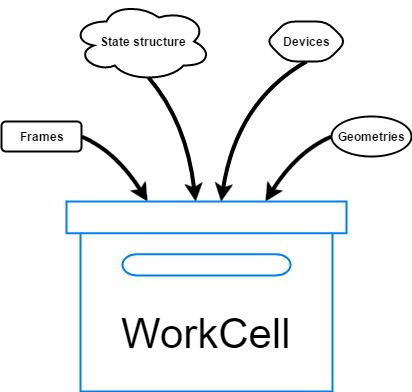
\includegraphics[scale=0.55]{Figures/WorkCellBoxExample.png}
	\caption{The WorkCell can be seen as a box containing the elements necessary to represent an environment}
	\label{fig:WorkCellBoxExample}
\end{figure}


\subsection{Frames}
One of the most common data structures from the RobWork library is a frame. A frame is the basic building block in the RobWork library, representing (in the case of RobWork) a local 3D euclidean space. In RobWork frames are built in sequence to each other to form the environment. This means that all frames have a parent and potentially children.\\

In RobWork frames come in 3 different types: fixed frames, moveable frames and joints.\\
Fixed frames are frames that have a constant transform relative to the parent frame.\\
Movable frames are frames which transform can be freely changed.\\
Joints are frames that can be assigned values for position, velocity limits and acceleration limits. This type of frame is usually used for devices. Joints can be further divided into 3 subtypes: prismatic joint, revolute joint and dependent joint.\\
Prismatic joints are joints which motion is linear along a constant direction. Thinking of a pneumatic piston can be an intuitive way of thinking about prismatic joints.\\
Revolute joints are joints which motion is based on a rotation around a single axis. Thinking of hinges can be an intuitive way of thinking about revolute frames.\\
Dependent joins refer to joints which transform depends on one or multiple other joints. Dependant joins can also be divided into 2 subtypes, dependent prismatic joints and dependent revolute joints, adding the motion specification of the prismatic joint and revolute joint previously mentioned.\\

Frames in a WorkCell are required to have a parent and are given a unique name so that no frames can be confused for another. Only one frame in the WorkCell has no parent. This frame is called WORLD and is created when the WorkCell is constructed. The WORLD frame can be seen as the global 3D euclidean space for the WorkCell.


\subsection{Objects}
Contrary to frames which represents the relationships in the environment, objects represents physical things in the scene. Also contrary to frames is that the name of an object does not have to be unique.\\

In order for objects to get a relationship to the environment it is placed in, it has to be associated to a frame. This frame is called the base frame of the object. An object can be associated to multiple frames but only have one base frame.\\

An object consists of two important elements, a geometry and a model.\\
A geometry is used to represent the actual geometry of the object. The geometry can be scaled and transformed to allow for modifications. In order to perform a transform, the geometry need a reference. This is done with having the reference be a frame, a reference frame. RobWork is capable of creating simple geometries like spheres, boxes and cylinders, however it is also possible to import complex geometries. Geometries are also being used for the collision detection provided in RobWork.\\
A model is a graphical representation of the object. Models consists of geometries, materials, colors and texture information as well. It is also possible to apply a transform to a model and get the transform of a model.\\
Usually when an object is created, a geometry is created for collision detection and a model is created to visually represent the object in a viewer(e.g. RobWorkStudio).\\

There are two types of objects in RobWork, rigid objects and deformable objects. Rigid objects are objects which  geometry does not change. Rigid objects can also posses information about inertia and mass. A deformable object however has the ability to alter its geometry via control nodes.


\subsection{Devices}
A device can be considered a description of a arbitrary device e.g. the FANUC LRM200 robotic arm (Seen on figure~\ref{fig:FANUCLRM200}). The device also contains the configurations for the device it represents. These configurations are contained in a single configuration vector, making it easy to control the device. In case of a joint device (like the FANUC LRM200), it is also possible to get and set the bounds, velocity limits and acceleration limits for the joints.\\

\begin{figure}[h]
	\centering
	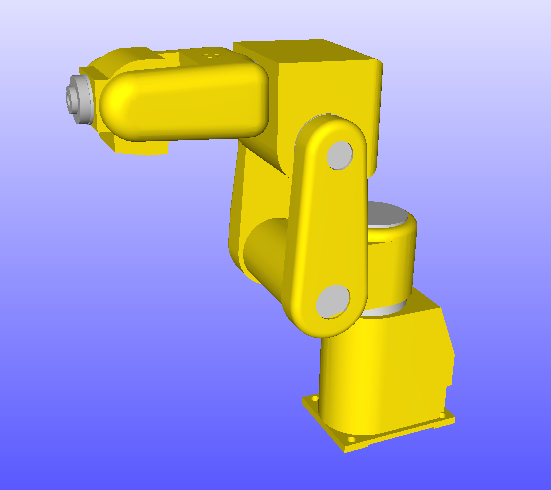
\includegraphics[scale=0.55]{Figures/FANUCLRM200.png}
	\caption{Model of a FANUC LRM200 in RobWorkStudio}
	\label{fig:FANUCLRM200}
\end{figure}

Devices can be of 3 different types: joint device, mobile device and SE3 device. Mobile devices are devices that  is differentially controlled e.g. a robot rover. Joint devices are devices that consists of moving joints much like the previously mentioned FANUC LRM200 robotic arm. SE3 devices are devices that can move in a 3D euclidean space and is not consisting of joints e.g. a drone.\\

Joint devices can be of 5 types: Serial devices, tree devices, parallel devices, composite devices and composite joint devices.\\
Serial devices are the simplest form of device since it consist of joints set in serial to each other. Many simple robotic arms like the before mentioned FANUC LRM200 are serial devices.\\
Tree devices are devices which joints follow a tree structure, meaning that a joint can have multiple children but only one parent joint. This also means that a tree device must have more than one end effectors. This type of device is typically seen in dexterous hands.\\
Parallel devices are devices that at some point in the structure, of the device, is created a circle e.g. a joint goes to two joints that then both go to the same joint. The two middle joints are said to be in parallel to each other and are called parallel legs in RobWork. Parallel legs can consist of multiple joints as well as just one.\\
Composite devices and composite joint devices are devices that are constructed from a series of other devices. The devices in the composite device may not share joints. Just like tree devices, composite devices can have multiple end effectors. However unlike the tree devices, composite devices does not require the path to the end effectors to have a common base. The difference between composite devices and composite joint device is that the devices used in a composite joint device needs to be of the joint device type, whereas in a composite device this is not a requirement.\\
Illustrations of the joint device types can be seen on figure~\ref{fig:DeviceTypes}.

\begin{figure}[h]
	\centering
	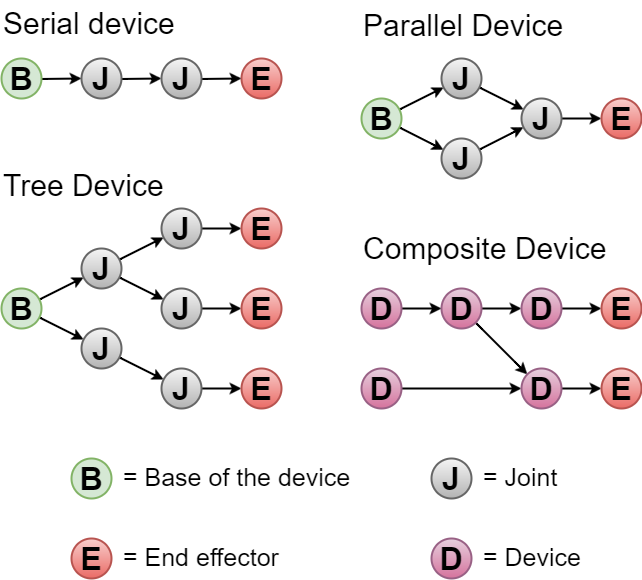
\includegraphics[scale=0.55]{Figures/DeviceTypes.png}
	\caption{The WorkCell can be seen as a box containing the elements necessary to represent an environment}
	\label{fig:DeviceTypes}
\end{figure}


\subsection{States and State Structures}
In RobWork the structure of the frames are represented through a class called State Structure. The State Structure also holds the state of all the frames in the form of a class called State. The State is a collection of the states of all the frames contained in the State Structure. This is done as a kinematic tree.


\subsection{Namespacing in RobWork}
The RobWork library is neatly divided into sections. Some of the more used sections are kinematics, models, geometry, loaders and math. When writing code using the RobWork library the namespace of the class one would want to access is the same as division of the library. As an example, accessing the the frame class from the kinematics section would be done like rw::kinematics::Frame. This makes it easier to locate the implementation of a class or fuctionality e.g. the implementation of the frame class is in the kinematics folder.\\

Most of the functionalities in RobWork are implemented as static functions. This makes coding with the RobWork library more intuitive since for some of the functionalities in RobWork it does not make sense to require an object to access the functionalities. As an example, accessing the load function of the XMLRWLoader (which loads in a XML-file describing the WorkCell) can be done simple by writing rw::loaders::XMLRWLoader::load(input for function), instead of creating a object of the XMLRWLoader and then calling load on the object.


\subsection{Typical use of RobWorkStudio and WorkCell-files}
Typically when using RobWorkStudio, the user create a WorkCell file written in XML. This file contains the necessary information for creating a WorkCell. The WorkCell file can then be loaded into RobWorkStudio by using the open button. The WorkCell file can also be loaded manually with the before mentioned XMLRWLoader returning a WorkCell object. When creating a WorkCell file it is necessary to know the tags used by RobWork. The root element in a WorkCell file is the WorkCell tag. The WorkCell tag should be written with the attribute name, giving the WorkCell a name. Inside the WorkCell tag different tags can be used to add the elements of the WorkCell. Some of the more common tags used are: frame, RPY, pos, joint, geometry tags, device tags and the include tag.\\
The frame tag is used to define a frame in the structure. The frame tag needs to be supplied with a name attribute and a type attribute defining the frame type.\\
The RPY tag is used within the frame tag to define the rotation of the frame and the pos tag is used to define the displacement. A transform can be used instead of these if the transform is available.\\
The joint tag is representing a frame of the type joint. This tag also needs a name attribute and a type attribute to define the type of joint.\\
There are also some simple geometry tags that are used for define simple geometries like a box. More complex geometries can be included via a polytype tag taking in the path for the model file.\\
Devices can be defined using different tags that define the different kind of devices in RobWork. As an example the serial device FANUC LRM200 would have a serial device tag with joint tags inside.\\
The include tag is used to include another XML file's content. This is usually used to include complex devices into an environment. This allows users to create only one description of a device and then include it whenever it is used. An example of a WorkCell described in XML can be seen in figure~\ref{fig:XMLCodeExample}.

\begin{figure}[h]
\centering
\lstset{language=XML} 
\begin{lstlisting}[frame=single]
<!-- WorkCell with the name attribute set to Scene -->
<WorkCell name="Scene"> 

<!-- New Frame called Table added to the World frame -->
  <Frame name="Table" refframe="WORLD" >
	<!-- Transform of the Table frame -->
    <RPY>0 0 0</RPY><Pos>0.2 0.2 -0.408</Pos> 
  </Frame>
  
<!-- New model named Table added to the Table Frame -->
  <Drawable name="Table" refframe="Table" >
	<!-- Transform of the model Table -->
    <RPY> 0 0 0</RPY> <Pos> 0 0 0 </Pos>
	<!-- Model information (box) of the model -->
    <Box x="0.8" y="0.8" z="0.816" />
  </Drawable>

<!-- New Frame called URMount is added to the frame Table -->
  <Frame name="URMount">
	<!-- Transform of the URMount frame -->
    <RPY>90 0 0</RPY><Pos>0 0 0</Pos> 
  </Frame>
  
<!-- Include the UR robotic arm from another xml file -->
  <Include file="../../XMLDevices/UR-6-85-5-A/UR.wc.xml" />	

</WorkCell>			 
\end{lstlisting}
\caption{Example of a WorkCell written in XML containing a UR robotic arm on a table. This example is from the examples following the the RobWork library (ModelData/XMLScenes/RobotOnTable)}
\label{fig:XMLCodeExample} 	
\end{figure}


\clearpage

\section{Qt}
%short introduction to the chapter
Qt, pronounced "cute", is an open source cross-platform framework, mostly used for GUI(graphical user interface) programming. Qt has an easy to (re)use API(application programming interface), which in return gives high developer productivity. QT is C++ class library, hence new developers using Qt should have some understanding of C++.
This chapter introduces terminologies used in Qt, and tries to give some general insight to how Qt operates and works regarding GUI development. For more information please refer to \cite{QtDocumentation}.

%Maybe something about licencing and version used.


%somewhere here should the "simple" inheritance diagram be.

\subsection{Qt Class Hierarchy and Object Model}
\label{sec:QtClassHierarchyAndObjectModel}
Qt broadly uses inheritance to create subclasses of instances in a natural way. QObject is the most basic class in Qt, see FIGURE. A lot of classes inherit from QObject, like QWidget, which is the base of all user interface objects. 
C++ offers efficient runtime for a object oriented scheme, but lacks in regard to flexibility due to the static nature of the C++ Object Model. Qt has implemented the QObject as the hearth of the Qt Object Model, which preserve the efficient runtime while also offering more flexibility for the GUI domain. The Qt Object Model is implemented with standard C++ techniques. Some of the features that the Qt Object Model adds are e.g.

\begin{itemize}
\item Inter-Object Communication called Signal and Slots in the Qt Object Model. This topic is expanded upon in section~\ref{sec:signalandslots}.
\item Object Trees which structures ownership of objects in a natural fashion. This topic is expanded upon in section~\ref{sec:qwidgets}.
\end{itemize}

\subsubsection{The Meta-Object System}
Due to the Qt Object Model the Meta-Object System was in turn created, which on the bottom line provides the Signal and Slots for inter-object communication and other features from the the QT Object Model. The Meta-Object System is based on three things:
\begin{enumerate*}[label={\alph*)},font={\color{red!50!black}\bfseries}]
\item the QObject class
\item the Q\_OBJECT macro and
\item the Meta-Object compiler(moc).
\end{enumerate*}
Each QObject or subclass of QObject has an instance of QMetaObject created to hold the meta-data information, e.g. the name of the class or the class's meta-methods(signal, slots and other member functions). The Q\_OBJECT macro helps and defines the meta data for the moc at compile time. Please refer to figure~\ref{fig:QtC++BuildProcess} to see influence of the Meta-Object System in compile time.

\begin{figure}[h]
	\centering
	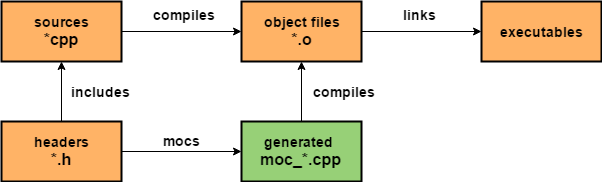
\includegraphics[scale=0.55]{Figures/QtC++BuildProcess.png}
	\caption{This figure shows how the the Meta-Object System is integrated at compile time. The yellow boxes indicate the normal C++ compiling procedure, whereas the green box is the added moc, which is compiled into the object files}
	\label{fig:QtC++BuildProcess}
\end{figure}

\subsection{QWidgets}
\label{sec:qwidgets}
QWidget is the base of all user interface objects(buttons, menus etc.). QWidget handles all events from the system the application is running on, i.e. In Qt, events are QEvent objects which is created upon outside activity (like a click on a mouse). Subclasses of QEvent involve more parameters to characterize a certain event, e.g. mousePressEvent(QMouseEvent* event). The event object is then sent to a specific QWidget object (maybe a button) and the QWidget handles the event with the according event handler.\\

As mentioned in~\ref{sec:QtClassHierarchyAndObjectModel} ownership of objects is structured in a tree, this means that a QWidget can have QWidget's within it self, see figure~\ref{fig:QWidgetExample}. A QWidget with no parent is called a top-level widget, which means the QWidget is an independent window. An instance like QWidget subclass QDialog(a pop up dialog window) is a top-level widget. QDialog can be instantiated with a parent, but the QDialog is still a top-level widget in this case, though the position of the dialog window is now centred relative to the parent.

\begin{figure}[h]
	\centering
	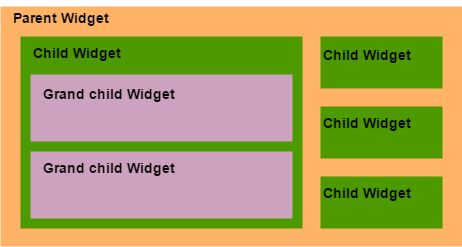
\includegraphics[scale=0.55]{Figures/QWidgetExample.png}
	\caption{Qt structures ownership of objects in a parent child relationship. The diagram shows a parent widget with various child widgets in a layout, more on layouts in section~\ref{sec:QLayout}.}
	\label{fig:QWidgetExample}
\end{figure}

When a QWidget is used as a container to hold and group children, the QWidget is called a composite widget. A parent widget is clipped to the size that it children requires, though this can be changed in the widget's size policy. 

\subsubsection{QMainWindow}
QMainWindow is a subclass of QWidget, and is very essential to a Qt GUI application, since the QMainWindow is a framework for the application user interface. As seen on figure~\ref{fig:QMainWindowExample} a QMainWindow can have a menu bar widget, toolbar bar widgets, docked widgets and a status bar widget, though a QMainWindow must have a central widget, even if that widget is only a empty placeholder. 

\begin{figure}[h]
	\centering
	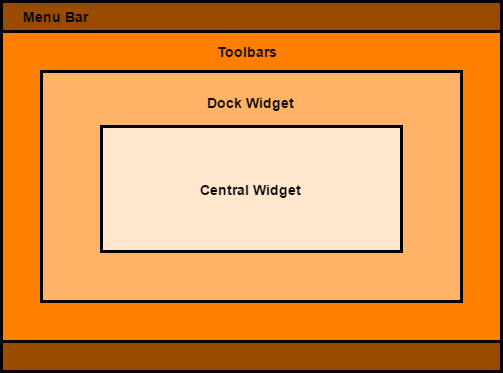
\includegraphics[scale=0.55]{Figures/QMainWindowExample.png}
	\caption{This figure shows how a QMainWindow object looks like. RWS uses QMainWindow as the main application widget.}
	\label{fig:QMainWindowExample}
\end{figure}

QMainWindow is usually a good class to use as the framework for an GUI application, though it is optional whether to use it or not. In the case of RWS, QMainWindow is used, and figure~\ref{fig:QMainWindowExample} nicely reflect the structure of RWS' GUI, where the central widget is a custom subclassed QWidget using Qt GUI modules providing classes for OpenGL integration for graphic rendering. Various plug-ins to RWS are available to be docked in the docking area, or to be top-level windows (more on plug-ins in section~\ref{sec:plugin}) and tool bars and a menu bar are present as well for use.

\subsubsection{QLayout}
\label{sec:QLayout}
QLayout is a subclass of QObject and QLayoutItem and is the base class of geometry managers. QLaoyt and it's subclasses are managers for the layout of a group of widget laid out in an application. All QWidget subclasses can use layouts to manage it's children e.g. figure~\ref{fig:QWidgetExample} uses the parent widget as composite widget with two composite children. The parent on figure~\ref{fig:QWidgetExample} use a QHBoxLayout, which lines the child widgets horizontally and makes each child fill one box. The children then has their own QVBoxLayout, which lines their children (grand children) vertically and assign each of those their own box as well. Figure~\ref{fig:QLayoutCode} shows how an implementation of five arbitrary widgets laid in the layout as in figure~\ref{fig:QWidgetExample}.

\begin{figure}[h]
\centering
\lstset{language=C++} 
\begin{lstlisting}[frame=single]  
QWidget* parent = new QWidget();  			//Parent widget
QHBoxLayout* pL = new QHBoxLayout();		//Layout of the parent widget
QWidget* cL = new QWidget(parent); 			//Left child widget
QVBoxLayout* cLL = new QHBoxLayout();		//Layout of left child widget
QWidget* cR = new QWidget(parent); 			//Right child widget
QVBoxLayout* cRL = new QHBoxLayout();		//Layout of right child widget
pL->addWidget(cR); pL->addWidget(cR);		//add children to layout
parent->setLayout(pL);						//set layout
QWidget* b1 = new QWidget(cL), b2 = new QWidget(cL), b3 = new QWidget(cR),
		 b4 = new QWidget(cR), b5 = new QWidget(cR); //create grandchildren
cLL->addWidget(b1), cLL->addWidget(b2);	//grand children added to layout
cL->setLayout(cLL);					//set layout
cRL->addWidget(b3), cRL->addWidget(b3), cRL->addWidget(b5);				 
cR->setLayout(cRL);			 
\end{lstlisting}
\caption{write stuff}
\label{fig:QLayoutCode} 	
\end{figure}


\subsection{Signal and Slots}
\label{sec:signalandslots}
Communication -> objects
Alternative to callback -> explain callback
Signal and slots -> connect() RET TO FIGURE
Signal -> 
Slot -> normal function (only special thing is it can be connected to a signal) -> found by moc
\subsubsection{Difference between events and Signal/Slots}

\subsection{Plug-in}
\label{sec:plugin}


\clearpage

\section{Describe functionality the user needs, and sort in order of importance}

\begin{itemize}

\item Loading objects into the WC, this does not necessarily mean with a drag like motion, but rather as a proof of concept without regards to the GUI.

\item Simple browser for objects.

\item Improvement of the GUI, this means adding a drag and drop-like feature to the GUI, where the user would drag an object from the object browser window into the WC.

\end{itemize}
\clearpage

\section{Inserting frames and geometries}
\label{sec:iframAGeom}
This section contains the description of the implementation of inserting frames and geometries. This is done trough a class called creator we made specifically for creating RobWork specific objects without a XML file description.

\subsection{General explanation of the solution}
\label{subsec:iFramesAGeomsGE}
The solution to the requirements related to insertion of frames and geometries was condensed into two parts, a user interface for the information needed (GUI) and the actions needed to insert the frames with the informations gotten from the user interface. In order to simplify the process of inserting frames and geometries, with the information given, this was separated into an extension to the RobWork library. The name chosen for this extension was creator since its focus was on creating and adding elements from the RobWork library.\\

Separating the problem into the GUI and creator have several benefits. First of all, it has the benefit of modularity. The creator is not dependant on a the GUI and is written in a way that allows use in other applications than this one.\\
Another reason is that it makes it easier to divide the task as long as the the information needed is agreed upon.

\subsection{Using the creator}
\label{subsec:iframAGeomUsing}
The creator follows the same namespacing technique as RobWork employ in order to make it more intuitive to use next to RobWork. However instead of using rw as the first namespace, ei (for EasyInsert) is used. This could be changed to rw in order make the blend perfect, however it was chosen not to in order to make the user aware that the creator is not part of the official RobWork library.\\

In the case of frames, the creator is capable of creating fixed frames and movable frames. The creator is also able to add them to a supplied WorkCell and in the case of the movable frame, give it an initial transform in the WorkCell. The fixed frame should always be supplied with a transform, since this is a criteria for the fixed frame type. 
Both functionalities returns a handle to the newly created frame which the user can user instead of being forced to search the WorkCell for a handle after creating the frame.\\

In the case of geometric primitives, the creator is capable of adding 6 different geometric primitives to a specified WorkCell: boxes, planes, spheres, cones, cylinders and tubes. No matter what geometric primitive the user wishes to create, the user needs to provide the WorkCell. The user also needs to provide a pointer to the frame they wish to include the geometric primitive to. Instead of this the user can supply the name of a parent frame for a new movable frame on which the geometric primitive is put. The user also needs to provide the necessary information in order to create the different geometric primitives. This varies between the different geometric primitives, a list of the different inputs need for the different geometric primitives can be seen on figure~\ref{fig:InputsForGeoms}. It is also possible to supply the function with a transform which then represents the local transformation of the geometric primitive in relation to the frame on which it has been included.\\

\begin{figure}[h]
	\centering
	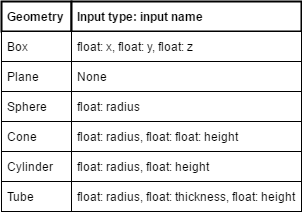
\includegraphics[scale=0.55]{Figures/InputsForGeoms.png}
	\caption{Table of geometric specific inputs for the individual geometric primitives}
	\label{fig:InputsForGeoms}
\end{figure}

Since a lot of transformations are used in the creator it was decided also to create a function to easily create transform objects from R,P,Y and x,y,z values. The function, called getTransform3D, takes in these values and returns a Transform3D object.\\

An example of adding a sphere to a new WorkCell can be seen on figure~\ref{fig:CodeExampleAddSphere}.

\begin{figure}[h]
	\centering
	\lstset{language=C++} 
	\begin{lstlisting}[frame=single]
	// Create new wc
	WorkCell::Ptr dummy = ownedPtr(new WorkCell("wc"));
	 
	// Radius of 10 cm
	float radius = 0.1;
	
	// Displacement of 10 cm in x, y and z
	Transform3D<double> transform = getTransform3D(0.1, 0.1, 0.1, 0, 0, 0); 
	
	// Adding sphere to WorkCell
	ei::creator::addSphere( "testSphere", // Name of Sphere
							"WORLD", // Name of parent frame
							wc, // Pointer to WorkCell
							radius, // Radius of Sphere
							transform); // Transform of Sphere
	 
	\end{lstlisting}
	\caption{Code example of adding a sphere to a new WorkCell. The sphere has a radius of 10 cm and a displacement of 10 cm in x, y and z in relation to the frame on which it is set. The sphere is added to a new movable frame with the parent set to the WORLD frame.}
	\label{fig:CodeExampleAddSphere}
\end{figure}

\subsection{Implementation of the creator}
The creator was implemented with the purpose of using the most upper layers of the RobWork libraries functions to solve as much of the problem as possible. This was done since in RobWork it is possible to access lower levels of the library which makes the RobWork library way more flexible. An example of this could be when working with the frames of a WorkCell the upper layer way of doing it would be accessing the frames through the WorkCell's own functionality for getting frames, whereas the lower layer of doing it would be to access the state structure in the WorkCell and through it access the frames. The other reasoning for using upper layers is that it is usually simpler code, meaning there is less mistakes to make and the mistakes made are easier to find.\\

The implementation of the getTransform3D function is rather simple since it utilises some conversions in the RobWork library. The inputs for the function are 6 doubles representing the x, y, z values, which is the displacement, and the R, P, Y values representing the rotation. In order to create a Transform3D object, a vector representing the displacement and a matrix representing the rotation is needed. The displacement vector is easy to create since it is just a vector containing the x, y, z values directly from the input. The rotation matrix however is more difficult to get since the input for the rotation is represented in R, P, Y values. The R, P, Y values needs to be converted to a rotation matrix. Instead of doing the calculations manually, RobWork, albeit a little hidden, can do this for us through the RPY class from the math namespace. First an RPY object is created with the values from the input. Then the member function toRotation3D from the RPY class is called returning the rotation matrix of the given R, P, Y values. The displacement vector and rotation matrix is then used to create a Transform3D object that is returned to the user. It would be possible to just implement the same functionality that the toRotation3D RPY class, eliminating the creation of an RPY object. This would increase the computation speed, but not significantly unless the function is used a lot.

\subsubsection{Implementation of creating and adding frames}
There are a total of 4 functions in the creator that are related to creating and adding frames to a WorkCell. The first 2, one for each type of frame, are functions related to creating frames. The implementation of creating frames in the creator is rather simple, since the process of creating frames in RobWork is simple in itself. The 2 functions are called createFixedFrame(...) and createMovableFrame(...). The createFixedFrame(...) function take the name of the frame and a transform as input, whereas the createMovableFrame(...) only takes the name as input. The functions simply call the constructor for the given frame with the provided parameters. The reasoning behind having these rather simple functionalities is in the context that the creator should be consistent in the functionality it embodies. Another good reason was that this was some of the first functionalities implemented for the creator. At the time the idea was that there would also be a function, atleast for the fixed frame, that took in the x, y, z and R, P, Y values instead of a transform. The function would then calculate the transform by itself and use this transform when creating the frame. This was however deemed unnecessary to implement when the getTransform3D(...) function was implemented.\\

The last 2 functions, again one for each type of frame, are functions that are capable of creating and adding a frame to a specific WorkCell. The two functions are called addFixedFrame(...) and addMovableFrame(...). Both of the functions take in a WorkCell, a name, a name of a parent frame and a transform. These functions eliminates the need for the user to understand how to create a frame and how to add the frame to the WorkCell. Even though one could say that this is rather simple process to learn, using the creator simplifies the process significantly. This comes at the cost of flexibility since the user is now locked to the implementation of the functions. However it was estimated that in many cases the functionality implemented in the creator could be used. Figure~\ref{fig:CodeExampleAddFrameDifference} showcases the standard way of creating a frame and the adding it to a WorkCell, versus using the creator.

\begin{figure}[h]
	\centering
	\lstset{language=C++} 
	\begin{lstlisting}[frame=single]

	string name = "test"; // Name of frame
	string parent = "WORLD"; // Name of parent frame
	Transform3D<double> transform =  // Transform used
	ei::creator::getTransform3D(1, 1, 1, 1, 1, 1);
	WorkCell::Ptr wc; // WorkCell

	/// The standard way of adding a frame ///
	
	// Create new movable frame object and cast to frame
	MovableFrame* mframe = new rw::kinematics::MovableFrame(name);
    Frame* frame = dynamic_cast<rw::kinematics::Frame*>(mframe);
    
    // Find the parent frame in wc
    Frame* parentFrame = wc->findFrame(parent);
	
	// Test for eligible parent
	if(parentFrame != NULL) {
	
		// Add the frame to the wc
        wc->addFrame(frame, parentFrame);
		
		// Get state of wc
		State state = wc->getDefaultState();
		
		// Set transform of the movable frame in the wc
		mframe->setTransform(transform, state);
		
		// Upgrade state and update state
		state = wc->getStateStructure()->upgradeState(state); 
		wc->getStateStructure()->setDefaultState(state); 
    }
	
	
	/// Using the creator ///
	ei::creator::addMovableFrame(wc, name, parent, transform);

	\end{lstlisting}
	\caption{Code example of the standard way of adding a movable frame with a transform and the same process using the creator}
	\label{fig:CodeExampleAddFrameDifference}
\end{figure}

\subsubsection{Implementation of creating geometries}
Since in RobWork a geometric primitive, like a box, is called an object, a way to create a object that contains the information to represent the geometric primitive is needed. Getting inspiration from the implementation of the RWXMLLoader (See section~\ref{subsec:XMLRWLoader}) in RobWork, it was chosen to use the same factory approach as the loader. This means that when creating the geometry part of the object, the GeometryFactory from the loaders part of RobWork is used. When the model part of the object is created the Model3DFactory is used, again from the loaders part of RobWork. All of this is neatly put into 3 functions, addObject(...), createGeom(...) and createModel(...).\\

In order to understand process of adding e.g. a box it is easiest to start from the bottom with what the factories need in order to produce the geometry and the model. From the GeometryFactory a function called load(...) is used. This function takes in a string containing the information about the geometry it needs to produce and a bool that signifies whether or not the user wishes to use cached geometries. As an example, the syntax for the string when creating a box is "\#Box dx dy dz", where dx, dy and dz are the dimensions of the box. The syntaxes for the rest of the geometries can be seen on figure~\ref{fig:SyntaxTable}. The function create createGeom(...) uses the GeometryFactory to create a geometry and return it.\\

\begin{figure}[h]
\centering
\begin{tabular}{|l|l|l|}
\hline
Geometry & Syntax                           & Explanation of parametres                                                                                                                    \\ \hline
Box      & "\#Box dx dy dz"                 & The dx, dy and dz are the dimensions of the box                                                                                              \\ \hline
Plane    & "\#Plane"                        & Planes need no parameters                                                                                                                    \\ \hline
Sphere   & "\#Sphere radius"                & The radius is the radius of the sphere                                                                                                       \\ \hline
Cone     & "\#Cone radius height"           & The radius is the radius of the cone and the height is the height of the cone                                                                \\ \hline
Cylinder & "\#Cylinder radius height level" & The radius is the radius of the cylinder, the height is the height of the cylinder and the level is the discretization level of the cylinder \\ \hline
Tube     & "\#Tube radius height level"     & The radius is the radius of the tube, the height is the height of the tube and the level is the discretization level of the tube             \\ \hline
\end{tabular}
\caption{Table showing the syntaxes for the different geometric primitives}
\label{fig:SyntaxTable}
\end{figure}

From the Model3DFactory a function called getModel(...) is used. This function takes in a string that either describes a geometry in the same syntax as the GeometryFactory or a file name. It also takes in a string representing the name of the model. It is rather beneficial that the input for describing the geometry is the same for both the GeometryFactory and the Model3Dfactory since it makes it simpler to implement. The function createModel(...) uses the model3Dfactory to create a model and return it. The function addObject(...) uses both the createGoem(...) and the createModel(...) functions when constructing the object.\\

The addObject(...) function now needs to be interfaced to the individual geometric primitives. It is also known that the addObject(...) needs to be supplied a string describing the geometry. To do this a series of easy to use functions related to the geometric primitives were created. An example of one of these is the addSphere(...) which takes in the necessary information to describe a sphere (the radius) and then creates the appropriate string for the factories. It then calls the addObject(...) function with this string, and other relevant information, which creates and adds the object to the WorkCell. An example of the function flow, using addSphere(...), can be seen on figure~\ref{fig:CreatorFlow}.

\begin{figure}[h]
	\centering
	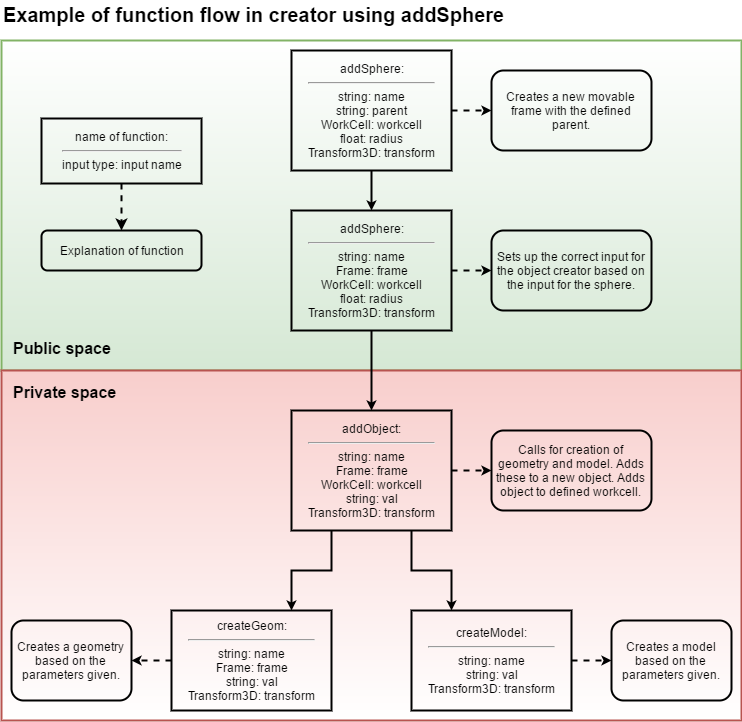
\includegraphics[scale=0.55]{Figures/CreatorFlow.png}
	\caption{Function flow of the creator using addSphere(...) as example}
	\label{fig:CreatorFlow}
\end{figure}

\subsection{The future of the creator}
Most of the functionalities that where implemented with the purpose to fulfil the requirements of the solution. The possibilities for the creator is however almost limitless. This is mostly due to the fact that the creator is written like a library extension to the RobWork library. One of the more immediate expansions to the creator that could be made, would be to extend the geometric primitive related functions with the possibility to only create the geometry or model when creating the object. This extension would make it possible to create visible objects with no collision or invisible objects with collision. Another good addition would be to create a functionality capable of loading geometries from a geometry file. This is already possible in RobWork, so it would make sense to also simplify this process in the creator.
\clearpage


%------------------------------------------------
% Litteraturliste
%------------------------------------------------
%\printbibliography

\begingroup
\sloppy
\hvisdansk%
	{\printbibliography[heading=bibnumbered,title=Litteratur]}%
	{\printbibliography[heading=bibnumbered]}
\endgroup

%	
%
%************************************************
% Bilag
\setcounter{BilagSider}{-\thepage}
%************************************************
\startbilag
\titleformat{\section}{\normalfont}{\Large\bfseries Appendix~\thesection}{15pt}{\Large\bfseries}

%\titlelabel{Appendix~\thetitle\quad}
%	
%
%------------------------------------------------
% Ord- og symbolliste 	Kan pt. kun bruges med report klassen
%------------------------------------------------
%	\let\stdchapter\chapter
%	\def\chapter*#1{\stdchapter{#1}\label{symbolliste}}
%	\printnomenclature[2cm]
%	\let\chapter\stdchapter
%
%************************************************
\addtocounter{BilagSider}{\thepage}
%************************************************
\end{document}